\section{LAMP optimisation techniques}\label{sec:lamp_optimise}
\begin{quote}
	\ldots Simplifications have had a much greater long-range scientific impact than individual feats of
ingenuity. The opportunity for simplification is very encouraging, because in all examples that come to
mind the simple and elegant systems tend to be easier and faster to design and get right, more efficient in
execution, and much more reliable than the more contrived contraptions that have to be debugged into
some degree of acceptability....Simplicity and elegance are unpopular because they require hard work and
discipline to achieve and education to be appreciated.

-- Edsger W. Dijkstra
\end{quote}

\subsection{What is LAMP?}
\gls{lamp} is a software bundle of free, open source software containing everything you actually need to run a fully working website for development or production environment. 
The first letters stand for Linux, Apache, MySQL and PHP (sometimes Python or Perl). 
The combinations of software included may vary but in our setup they're going to be \gls{apache} the webserver, \gls{mysql} the database and \gls{php} the dynamic interpreted language.
At the bottom there's GNU/Linux, Apache, PHP and MySQL are all applications on top of that. Apache communicates with PHP which makes the database connections with MySQL.

When a client sends a HTTP request to the \gls{apache} webserver it then looks up for what type of request it is. If the file is a simple statical HTML one, it just sends it to the client.
If it's a \gls{php} one then it makes use of the php5-module to communicate to \gls{php}. The \gls{php} interpreter then connects to the MySQL database. 
It isn't a persistent connection but a new connection every time so there is a lot of latency.  (\autoref{linux/lamp_stack.png} on page~\pageref{linux/lamp_stack.png}).

vApus simulates a lot of concurrent users to stresstest the \gls{lamp} settings (\autoref{linux/lamp_clients.png} on page~\pageref{linux/lamp_clients.png}).
\img[htb!]{scale=0.6}{linux/lamp_stack.png}{How the LAMP stack works}
\img[htb!]{scale=0.6}{linux/lamp_clients.png}{vApus and normal Client http requests}
\subsection{What is optimisation?}
\subsubsection{Not only about coding}
While there are a lot of websites that give good examples of code optimisation techniques not all the code
you can find is optimised. Many of these existing ,,techniques'' are mostly outdated when a new version
of a compiler and/or interpreter came out for a specific programming language. Coding equally has to
do with the style you have, most people mix all styles of coding. Because of this, we get unreadable huge
code bases for things that could be run simpler. If the code was somewhat better structured so it wouldn't
run too many useless functions per page view and actually run what you need instead of loading
everything, things would be much better. Using faster algorithms instead of implementing the same bad
function in C/C++ as an external library would improve. Preloading the most used functions in memory instead of loading them at each request.

It isn't always about the code, sometimes other parts of your system are the bottlenecks and it's up to the
programmer to fix them.\cite{phplens_optimising_tips}
\subsubsection{How to optimise?}
What we're after now is to find settings that aren't that hard to edit and get optimal speed without
requiring us to go deep into PHP code. So it will mainly be Apache and OS optimisations.

\subsubsection{The logic between speed versus accuracy versus scalability}
Grace Hopper the mother of \gls{cobol} and one of the pioneers in computer programming mostly made
references to the distance of electricity that passes through a wire in one microsecond. She joked that all
programmers should have a cable of 300 m around their necks\cite{graceHopper_story} and encouraged programmers not to even
waste one microsecond! In the beginning of computer age that was easy to understand why, computers
weren't as powerful as they are today. As far as everyone would say: ,,Premature optimisation is the root
of all evil'' and it's true if you have a good coding habit and everything is readable and not machine
dependent. But if you start writing spaghetti code it won't do you any help at all if you try to optimize it
later since you'll start wasting time. Always code with the best techniques in mind and you won't have to
optimize too much later.

It's impressive how they made the first flight to the moon with only 32 kB of \textbf{read-only} memory and
only 2k volatile.\cite{graceHopper_history}

People usually forget that performance is a set of trade-offs that a programmer must do between speed,
scalability and accuracy. One example is using caching where you mix accuracy with speed what means
that you either have up to date data or faster older data. Scalability or speed is achieved when people tend
to load everything into memory for speed but then their applications can't handle too many requests
especially in very used websites. The best thing that you can do is always use as less memory as you can.

\subsubsection{Bottlenecks}
Let's explain everything with one example where we're using two scripts that lets say both read one file
and then generate one html page: \textbf{loadwholefile.php} loads the whole file into memory and
\textbf{loadsmallparts.php} only loads one line at a time. Because of this, \textbf{loadsmallparts.php} will be slower
than the other one because it accesses the disk more times than needed.

The first one needs 0.05 \gls{cpu} time and 12 MB \gls{ram}, the second needs 0.08 cpu time and 5 MB RAM.
Let's say that in theory we have 128 MB of memory on that system, of which 8MB is used for the system
and that the processor is 99\% idle, which does really occur in reality when a system is not used.

Now \textbf{loadwholefile.php} will run out of memory when running 10 concurrent scripts and if more
concurrent requests are needed it will start using virtual memory (swap) and everything will slow down a
lot but \textbf{loadsmallparts.php} will still have 70 MB left for 10 concurrent scripts.\\
In the end we have something like this:

%\ANDREI START MAKING the tables here!
\begin{table}[ht!]
\caption{CPU usage of scripts}
\arrayrulecolor{myLightGreen}
\begin{tabular}{|p{4cm}|p{3cm}|p{3cm}|p{3.2cm}|}\hline\rowcolor{myLightGreen}
 {\bf\color{white} Scripts} & {\bf\color{white} CPU seconds for 1 HTTP request} & {\bf\color{white} CPU seconds for 10 HTTP requests} & {\bf\color{white} CPU seconds for 20 HTTP requests} \\ \hline 
 {\bf\color{black} Loadwholefile.php} & {\bf\color{black} 0.05} & {\bf\color{black} 0.5} & {\bf\color{black} 2 (no more ram)} \\ \hline 
 {\bf\color{black} Loadsmallparts.php} & {\bf\color{black} 0.08} & {\bf\color{black} 0.8} & {\bf\color{black} 1.6} \\ \hline 
\end{tabular}
\end{table}

Here we see that \textbf{loadwholefile.php} uses another 100 Mb of swap/virtual memory for the 20 requests and this is very slow while the \textbf{loadsmallparts.php} still has 20 MB RAM free and is faster in total.
Of course this is just an example, real world examples are different.
\myparagraph{Network}\\
Of course the network link is a bottleneck if you still use a 10 Mbit connection to serve a few clients with 50KB of content if you can only use 1 MB of the total. But since there already are 400Gbit processors out there\cite{400g_network_processor}  bandwidth shouldn't be the bottleneck and if you're using Gzipped content it should be even better. Distributed load handling could also help resolve most issues.
\myparagraph{Processor load}
With the new multi-core and multi-processor evolution this shouldn't be a problem unless you use \gls{php} to do intensive calculations that you'd better do in C/C++. Dynamic pages do use a lot of CPU in PHP but sending simple files isn't that bad. This is usually not the issue with performance unless you do on the fly video encoding on the webserver, and this isn't the case.
\myparagraph{File system}
Following the evolution of \gls{ram} and \gls{cpu} we see that the hard disk has become a black hole. Imagine that a disk seek is 3.3 ms, almost 3.300.000ns while DRAM runs at 300Mhz and it only uses 3.3 ns/cycle. Wow, one million times slower? Even 1000 times slower would be a big difference. Using Windows for a webserver also has the bad habit of getting your data fragmented, this doesn't happen under Linux.

Using \gls{ssd}'s for your database and for your \gls{php} scripts could improve the speed drastically.
\myparagraph{Threading and processes}
The creation of a new process is very slow, using multi-threaded systems is the best thing you can do but since PHP has only been thread-safe for a small time it's best to just remove unused services on your server.
\myparagraph{External services}
If your application/webserver needs to connect to an external service every time you need something it can be very slow if it's on the server side. If you do it on the client side otherwise, the client will not see too much of a difference.
\myparagraph{When do you optimise?}
There are wide and variable meanings on this and to be hones the best advice people could have is to know what type of application they require, do some hardware benchmarks to know how it should behave in the future and design it with those parameters in mind. Use the perfect mix between performance, security, usability, flexibility and availability and don't forget to keep it simple so it can \textbf{\underline{scale}} in the future.
\subsubsection{Techniques}
\myparagraph{Database}
This is one of the most important things to optimise. Storing images or binary data in it is a bad idea since it's a network request that could be slow. Firstly because the database needs time to find everything, and send it via the network to your application, then you need to make an image and send it. Optimise your queries for speed and be sure that you also examine the database configuration files if you can for optimisation. Don't use 500 MB for your DB if it's on a special server with 4 GB of RAM only for it alone!
\\Run multiple inserts in one query than in a for (each) loop!
\myparagraph{Caching}
Caching is one of the techniques to achieve high performance by not executing code but just showing an existing page. 
\\Blogs can just save \gls{html} files every time the editor edits a post and just serve that instead of just querying the database. Forums could just check the last edition time of a page/post and the last version of a cache and compare the two instead of always querying everything. 
\\You can set up expiry time; there are lots of solutions out there for caching.
\myparagraph{HTTP accelerators}
Splitting the actual dynamic data from static content is what an accelerator should do; this lowers the \gls{cpu} usage a lot.
\myparagraph{Profiling software}
There are a lot of profiling programs but the best is still Valgrind, we will discuss this later.
\subsection{RAID setup and content migration}
We'll be using the same server as in the HipHop test case.
Since the CPUs and memory are rarely the bottleneck in a 16 core and 8 GB \gls{ram} configuration it's best to use 2-3 Intel 2.5" X25-E SLC 32GB SSDSA2SH032G1GN SSD's in RAID 0 for speed. This is a SOFTWARE \gls{raid} setup and has been done with the help of \textbf{mdadm}(see \autoref{mdadm} ), the Intel Embedded ,,fakeraid'' provided by the server that we're using for testing wouldn't work too well. The reason it wouldn't work is because it would either only boot from the SSD RAID or not see it at all when looking at the SATA HDD where Linux was setup. 
Another reason not to use the Intel Embedded RAID was that once in a while one \gls{ssd} would just crash without reason, this didn't happen with the software RAID. There is a little CPU overhead for this software RAID but it can be neglected.

\subsubsection{Setup disks}
First we used fdisk to empty all data from existing disks. For the purpose of this document the commands haven't been included since everyone should know how to do that.
\myparagraph{Create RAID set}
\textbf{Mdadm}\label{mdadm}\cite{mdadmLink} is a Multiple Disks admin that is a very simple tool to create \gls{raid} from multiple disks, on Linux of course. 
The reason we don't use the LVM installation from the Ubuntu setup is that we won't need to add newer/bigger hard drives since this \gls{raid} is only for the \gls{mysql} database and \gls{php} files. 
Because of the problems the Chenbro Nehalem server has with the disk controllers we'll actually only use 2 HDD's.
Create our \gls{raid}\cite{mdadmLink2} drive with this simple command.
\begin{codelisting}
	mdadm --create --verbose /dev/md0 --level=0  --raid-devices=2 /dev/sdb /dev/sdc 
\end{codelisting}
View the details:
\begin{codelisting}
mdadm --detail /dev/md0
\end{codelisting}
Format the new \gls{raid} set:
\begin{codelisting}
mkfs.ext4 /dev/md0
\end{codelisting}
Export the details of the partition to the \textbf{mdadm.conf} file to remember the configuration after reboot:
\begin{codelisting}
mdadm --detail --scan > /etc/mdadm.conf
\end{codelisting}
Create a mount point for \textbf{/dev/md0} and 
\begin{codelisting}
mkdir /mnt/raid
\end{codelisting}
Edit the \textbf{/etc/fstab} file to mount it on boot.
\begin{codelisting}
/dev/md0      /mnt/raid     ext4    defaults    1 2
\end{codelisting}
Finally mount it.
\begin{codelisting}
mount /dev/md0 /mnt/raid
\end{codelisting}

\subsubsection{Problems}
After setting hardware Intel Embedded \gls{raid}, one \gls{ssd} didn't work anymore. After setting software RAID in Linux, another one didn't want to work anymore. I think the controller is faulty. Problems while starting Linux because the ``RAID was corrupt or invalid''. BusyBox kept starting so eventually to fix the /etc/fstab (not even possible in recovery console) problem I had to take out all the \gls{ssd}'s and use 2 \gls{ssd}'s instead of one.
\\Now, at start-up the \gls{raid} set isn't mounting \textbf{/dev/md0} because somehow it's just seeing \textbf{/dev/md/chenbro-nehalem:0} instead, so we just alter the \textbf{/etc/fstab} file:
\begin{codelisting}
	/dev/md0      /mnt/raid     ext4    defaults    1 2
\end{codelisting}
\subsubsection{MySQL migration to SSD}
To be able to fully make a profit from 2 \gls{ssd}'s in \gls{raid} we need to do a migration of our \gls{mysql} databases so it runs faster.
Make the directory on the RAID SSD's, and copy the MySQL data to the new location. This data contains our databases.
\begin{codelisting}
mkdir /mnt/raid/mysql
cp -Rp /var/lib/mysql /mnt/raid/
\end{codelisting}

Edit the \gls{mysql} configuration file /etc/mysql/my.cnf.
\begin{codelisting}
	sudo vim /etc/mysql/my.cnf
datadir 		= /mnt/raid/mysql
\end{codelisting}

From Ubuntu 7.10 forward, Ubuntu uses a new security software AppArmor that specifies the areas of your filesystem that most applications are allowed to access. Modifying \gls{mysql} configuration without making changes to AppArmor means that MySQL won't restart and thus not work at all. Copy the two lines containing \textbf{/var/lib/mysql} copy them below and change them with \textbf{/mnt/raid/mysql} now it should work.
\begin{codelisting}
	sudo vim /etc/apparmor.d/usr.sbin.mysqld
\end{codelisting}

Restart the AppArmor profiles with the following command:
\begin{codelisting}
	sudo /etc/init.d/apparmor reload
\end{codelisting}

Restart \gls{mysql} with this command:
\begin{codelisting}
	sudo service mysql restart
\end{codelisting}
Everything should work perfectly now.

\subsubsection{Apache migration to SSD}
It's of great importance that your website files are also read from \gls{ssd}'s as the access time can double and it's faster when more users are using it.
Just edit \textbf{/etc/apache2/sites-available/default} and  \textbf{/etc/apache2/sites-available/default-ssl} to include the following locations: 
\begin{codelisting}
4	DocumentRoot /mnt/raid/www
\end{codelisting}
Now restart apache, I created a test file called hello.html to test if it really does work. And it does.

\subsection{Optimisation tweaks and profiling}
First before anything else we need to know our tools and how to actually profile what we've done. 
Stress testing is an important step in finding what works best and what doesn't. We'll be using \gls{vapus} for this since it gives a full featured testing environment.

Profiling a website must be done on all possible ways starting from the Frontend to the Backend and everything in between ex. database, filesystem, operating system tweaks etc. In high traffic websites everything must be correctly estimated or else failure is not a good friend to live with.
\subsubsection{Frontend}\label{subsec:frontend}
Everyone's first step into the world of optimisation is the frontend, what the client receives and gets displayed for him. This is important because here we can make our further assumptions on what is going wrong and start a top-down analysis to find the bottleneck or the bad doers. We can easily see if a page is loading too long and we could think that maybe an image is missing or that a script is doing too much time. Or maybe the server settings are wrong when it comes to streaming.

Frontend optimisations are done in multiple steps and can be from simple settings to big patches or extra modules for \gls{apache} or \gls{php}.

Some examples include but are not limited to using compressed content (.css, .js) and having two different subdomains; one for the static content and another for the dynamic one. This increases the speed of downloading. Optimizing images to be of lower quality and increasing the cache values of all the files that get retrieved from the server. 

There are however many tools that give information on what needs to be done so everyone can search for their own. Two such free tools are \textbf{Google PageSpeed} and \textbf{YSlow}. Both of them do the same thing of giving information on what needs to be optimised. We'll use both since they complement each other and we have more information on what to do to improve our websites.
\\Both of them are installed as add-on's for Chrome.

\myparagraph{Google PageSpeed}
Google PageSpeed (see \autoref{rId38.png}) gives us a score of \textbf{77/100} and it's not bad at all, but it isn't perfect. The only bad thing we see is that we should edit the browser caching. 
\img[h!]{scale=0.41}{rId38.png}{Google PageSpeed in Chrome}

\myparagraph{YSlow}
YSlow (see \autoref{rId39.png} on page \pageref{rId39.png}) on the other hand gives us more information with specific Links to yahoo developer pages on what exactly we should do, even if it isn't telling us code to use the explaining they offer is great so we can search the internet for optimisation tricks.

A content delivery network would be nice to use, we can set one up on our own domain but since we don't offer too many images it isn't needed.

Our overall score here is \textbf{83/100} and this is great.
%the best way to keep the images together and still have the text where it should be:)
\img[h!]{scale=0.41}{rId39.png}{Yahoo YSlow in Chrome}
\newpage{}

\subsection{Xdebug PHP profiler}
One of the important steps is to profile the \gls{php} script you are using, but this could be left as the last step if you're more interested in simple optimisations for just a simple site.

When coding a project it's valuable to know which functions get to run most of the time and how many times they have been called. Also knowing how much \gls{cpu} time and memory one function uses is of great value. This is very helpful if you want to see what goes wrong, and what can be optimised. \textbf{Valgrind} is such a tool made for C/C++ and other applications.

\textbf{Xdebug} an equivalent for \gls{php} it uses \textbf{Valgrind} for the generation of files that contain the time needed for a page to be run and also the time per function. 

\textbf{KCacheGrind} is a graphical tool that imports valgrind/xdebug files and displays them in a very user friendly manner. You can view a lot of graphics and representations and quickly find out what's using everything, going from one function to the other; the possibilities of source code reviewing are superb. If you import the output file from a server on your workstation then you can just specify the local source code and you'll be able to view which code exactly is working "slow" without having to open each file.

\subsubsection{How to install Xdebug}
Xdebug is open source so you can get it from github.
\begin{codelisting}
git clone git://github.com/derickr/xdebug.git
Resolving deltas: 100% (8272/8272), done.
Cd xdebug/
./configure --enable-xdebug
make -j16
sudo make install
\end{codelisting}

\subsubsection{Configure PHP to use Xdebug}
First find the right php.ini that you want to use:
\begin{codelisting}
\$ Locate php.ini
/etc/php5/apache2/php.ini	
\end{codelisting}

Now add the last file to the php.ini. Reload the webserver.
\begin{codelisting}
echo 'zend_extension="/home/lostone/xdebug/modules/xdebug.so"' >> /etc/php5/apache2/php.ini
\end{codelisting}
Also add this:
\begin{codelisting}
;xdebug.profiler_output_dir="/home/lostone/xdebugprofile"
xdebug.profiler_append=On
xdebug.profiler_enable_trigger=On
xdebug.profiler_output_name="valgrind.%R-%u.trace"
xdebug.trace_options=1
xdebug.collect_params=4
xdebug.collect_return=1
xdebug.collect_vars=0
xdebug.profiler_enable=0
sudo service apache2 restart
\end{codelisting}

Definitions are explained below\cite{xdebug_website}:

\textbf{xdebug.profiler\_append = profiles} will not be overwritten within the same file

\textbf{xdebug.profiler\_enable\_trigger=On} this enables you to use GET/POST parameters in a request with the name XDEBUG\_PROFILE. This will write profiler data in your defined output directory and it prevents the profiler from generating profiles on each request so you won't have gigabytes of profiling data if other people request your webserver or you stresstest it.

\textbf{xdebug.trace\_options=1 }allows the traces to be appended to the file instead of overwriting it.

\textbf{xdebug.collect\_params=4} Collects and reports the full variable contents and variable names.

\textbf{xdebug.collect\_return=1 }returns the value of function calls in the trace files

\textbf{xdebug.collect\_vars=0} doesn't collect the info about variables used because this is quite slow as explained on the xdebug documentation because Xdebug needs to do reverse engineering.

The best way to do it is look into /tmp/ after the files you want because if you specify your own folder, it might not work as expected. Finding something that works has been very time consuming. The above text works almost everywhere. All we need to do now is go to a webpage and add a GET request of ?XDEBUG\_PROFILE to enable profiling of that script\cite{diagnose_php_with_xdebug}.
\begin{codelisting}
http://chenbro-nehalem/phpbb/index.php?XDEBUG_PHP
\end{codelisting}

We then find a file called /tmp/valgrind.\_phpbb\_index\_php\_XDEBUG\allowbreak{}\_PROFILE-1331719932\allowbreak{}\_493209.trace that we will import in KCachegrind to view it in more details:
\img[h!]{scale=0.4}{rId40.png}{KCacheGrind graphical functions overview on index.php}

What we can conclude from (\autoref{rId40.png} on page~\pageref{rId40.png}) is that 37\% of the time is spent in the \textbf{common.php} file.
At a closer look we see that some MySQL functions take a lot of time to initialise, \textbf{user-$>$setup} and \textbf{session-$>$session\_create.}

After looking for a while into the PHP documentation online\cite{php_session} we found out that we can use another \underline{session path} for our sessions. Since the phpoptimised is only for our machine for testing purpose we won't change the info in php.in. Instead we will make our changes into the file \textbf{/include/session.php}.
\begin{codelisting}
mkdir /mnt/raid/sessions
chmod 777 /mnt/raid/sessions
ini_set('session.save_path', "/mnt/raid/sessions" );
\end{codelisting}

After surfing to \url{http://192.168.35.35/.php?XDEBUG_PROFILE} and importing the generated file into KCacheGrind, we still see no difference(\autoref{rId42.png} on page~\pageref{rId42.png}).
After looking through the code, we see that the session takes a long time not because of the location of the changes but because of the time it's needed to build the SQL requests and to work with \gls{mysql}. This is the second time MySQL and SQL requests take a long time. The question is what do they do exactly, and are they really needed? That can be normal since every connection to a MySQL instance takes time. The phpBB developers must know what they're doing.
\img[!htb!]{scale=0.6}{rId42.png}{KCacheGrind information on session\_create}
\img[h!]{scale=0.4}{rId44.png}{KCacheGrind graphical functions overview on viewtopic.php}
Now let's try to view a new link, and see how that's like. This time we'll use viewtopic.php.
\url{http://192.168.35.35/phpbboptimised/viewtopic.php?f=7&t=3532&XDEBUG_PROFILE}

\newpage

\begin{comment}
	

\begin{wrapfigure}{r}{0.7\textwidth}
  \vspace{-20pt}
  \begin{center}
 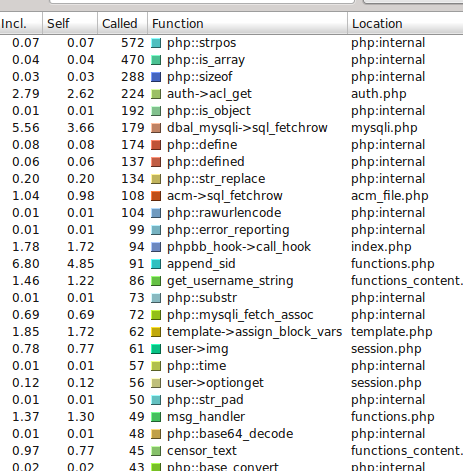
\includegraphics[scale=0.69]{rId45.png}
  \end{center}
  \vspace{0pt}
	\caption{Functions usage in KCacheGrind\label{rId45.png}}
  %\vspace{-10pt}
\end{wrapfigure}
\end{comment}
We see a different view this time, \textbf{common.php} (\autoref{rId45.png} on page~\pageref{rId45.png}) is using only 28\% of the time, the rest is for other things. Now let's see what functions are being used the most, and the time it takes for them to run. Maybe we can optimise something there. We can conclude that for one simple page request the internal strpos() function is ran almost 572 times. Since it's an internal function, and it doesn't use too many time it will be neglected, the same for the rest of the internals.
\img[h!]{scale=0.7}{rId45.png}{Functions usage in KCacheGrind}

\subsection{Conclusion}
Optimisation is not only about coding but also about avoiding bottlenecks. They can be numerous including network latency, processor load, file system speed.
Threading and processes creation, memory leaks, depending on external services is very slow if you require a lot of data.

There are a few techniques for databases, using caching instead of regenerating the same content. 
Remember to always reprofile your software using Valgrind or Xdebug.

Moving your \gls{apache} files and \gls{mysql} databases to a \gls{ssd} (or more if you want SSD RAID) helps avoinding disk latency.
